\section{Dwa wierzchołki, jedna krawędź}

Na samym początku rozważmy najprostrzy graf, czyli o dwóch wierzchołkach $u,v$ połączonych krawędzią. Za wierzchołek startowy wybierzmy $u$. Istnieją tylko dwa możliwe stany systemu: $(I,S)$ oraz $(I,I)$. Przejście ze stanu $(I, S)$ do $(I, I)$ następuje z prawdopodobieństwem $p$ w każdej jednostce czasu. Zatem czas zarażenia drugiego wierzchołka $X_v$ ma rozkład geometryczny, $X_v \sim \mathrm{Geo}(p)$. 

Rozważmy teraz rozkład $Y_t$. Mamy $\mathbb{P}[Y_t=1]=q^t$, bo próba zarażenia musiałaby nie udać się $t$ razy oraz $\mathbb{P}[Y_t=2]=1-q^t$. Stąd $\mathbb{E}[Y_t]=1\cdot q^t + 2 \cdot (1-q^t) = 2-q^t$. 

Jeśli chodzi o zmienną $Z$ to zachodzi $Z=\max\{X_u,X_v\}=X_v$ a więc również $Z\sim \mathrm{Geo}(p)$ oraz $\mathbb{E}[Z]=\frac{1}{p}$.


\section{Trójkąt}


Popatrzmy teraz na nieco większy graf — trójkąt. Niech jeden z wierzchołków będzie źródłem $s$, pozostałe zaś $u,v$. Aby poinformować $u$ musimy uzyskać sukces bezpośrednio od $s$ lub zarazić $v$ a potem $u$. Możemy zapisać więc $X_u = \min\{A,B\}$ gdzie $A\sim \mathrm{Geo}(p)$ oraz $B\sim \mathrm{NegBin}(2,p)$. Wiemy, że $\mathbb{P}[A\le t] =1-q^t$. Z kolei 
\begin{equation*}
\begin{aligned}
\mathbb{P}[B\le t]
&= \sum_{k=2}^{t} (k-1)\cdot p^2q^{k-2}= \frac{p^2}{q}\cdot \frac{q}{{(1-q)}^2}\cdot((t-1)q^t-tq^{t-1}+1) \\
&=1-q^t-tpq^{t-1}
\end{aligned}
\end{equation*}
gdzie skorzystaliśmy z \Cref{summ:geo_1}. Dalej, z \Cref{fact:min_CDF} mamy
\[
    \mathbb{P}[X_u\le t] = 1 - (1-(1-q^t))\cdot (1-(1-q^t-tpq^{t-1})) = 1-q^{2t}-tpq^{2t-1}
\]

Jeśli chodzi o liczbę zainfekowanych po $t$ krokach, to skoro mamy trzy wierzchołki to i trzy wartości do policzenia. Oczywiście $\mathbb{P}[Y_t=1]=q^{2t}$. Aby po $t$ chwilach tylko dwa węzły był zainfekowane musimy zarazić któryś z wierzchołków po $1\le k\le t$ rundach z prawdopodobieństwem $2pq\cdot q^{2\cdot(k-1)}$ a następnie uzyskać $t-k$ porażek. Na każdą z nich mamy szanse równą $q^2$. Podsumowując 
\[
    \mathbb{P}[Y_t=2]=\sum_{k=1}^{t} 2pq\cdot q^{2\cdot(k-1)} \cdot q^{2\cdot(t-k)} = 2tpq^{2t-1}
\]
Na koniec mamy $\mathbb{P}[Y_t=3]=1-q^{2t}-2tpq^{2t-1}$. Ponadto
\[
    \mathbb{E}[Y_t] = 1 \cdot q^{2t} + 2 \cdot 2tpq^{2t-1} + 3\cdot (1-q^{2t}-2tpq^{2t-1}) = 3-2q^{2t}-2tpq^{2t-1}
\]
Widzimy, że $\mathbb{E}[Y_t] \to 3$ przy $t\to \infty$ co jest zgodne z intuicją.

Propagacja może sie zakończyć na dwa sposoby. Pierwszym z nich jest sytuacja, w której przez $t-1$ żadne zakażenie nie zaszło a w chwili $t$ zarażą sie oba wierzchołkie. Prawdopodobieństwo tego przypadku wynosi $p^2q^{2\cdot(t-1)}$. Druga możliwość to taka gdzie w $k$'tym kroku (dla $1\le k\le t-1$) zaraził się jeden wierzchołków, szansa $2\cdot pq\cdot q^{2\cdot(k-1)}$,  a potem przez kolejne $t-1-k$ kroków trzeci nie został zarażony, na co mamy prawdopodobieństwo ${(q^2)}^{t-1-k}$, do chwili $t$. To ostatnie przejście ma $1-q^2$ szans. Łącznie dostajemy
\begin{equation*}
\begin{aligned}
\mathbb{P}[Z=t]
&=p^2q^{2t-2}+\sum_{k=1}^{t-1} (2pqq^{2k-2})\cdot (q^{2t-2k-2}) \cdot (1-q^2) \\
&=p^2q^{2t-2}+2pq^{2t-3}\cdot(t-1)(1-q^2) 
\end{aligned}
\end{equation*}
Mamy też $\mathbb{P}[Z>t]=\mathbb{P}[Y_t\ne 3] = q^{2t}+2tpq^{2t-1}$. Wartość oczekiwana więc wynosi:
\begin{equation*}
\begin{aligned}
\mathbb{E}[Z]
&=\sum_{t=0}^{\infty} \mathbb{P}[Z>t]=\sum_{t=0}^{\infty} q^{2t}+2tpq^{2t-1} \\
&=\frac{1}{1-q^2}+\frac{2p}{q}\cdot \frac{q^2}{{(1-q^2)}^2}=\frac{-3q^2+2q+1}{{(1-q^2)}^2}=\frac{4-3p}{p{(2-p)}^2}
\end{aligned}
\end{equation*}
Wykonaliśmy dość sporo obliczeń jak na tak mały graf. Możemy zauważyć więc, że istnienie cykli w grafie znacząco komplikuje sytuacje jeśli chodzi o model SI \@. 


\section{Grafy ścieżkowe}

Jako pierwszą rodzinę grafów rozważmy grafy ścieżkowe $\mathrm{P}_n$. Załóżmy, że proces zaczyna się w wierzchołku $s=1$. Zatem infekcja rozchodzi się po grafie ``od lewej do prawej''. Dla tej rodziny grafów uda nam się wyznaczyć dokładny rozkład prawdopodobieństwa. Zauważmy, że czasy zarażenia kolejnych wierzchołków tworzą ciąg zmiennych losowych
\[
X_1 = 0, \quad X_{v} = X_{v-1} + U_k, \quad v\in\{2,3,\dots,n\},
\]
gdzie $U_2,U_3,\dots,U_n \sim \mathrm{Geo}(p)$ oraz $U_2,U_3,\dots,U_n$ są niezależne. 
Widzimy zatem, że $X_v \sim U_1 + U_2 + \cdots + U_{v-1}$ a więc z \Cref{fact:sum_of_geo_RV} $X_v$ ma rozkład ujemny dwumianowy, 
\[
X_v\sim \mathrm{NegBin}(v-1, p).
\]
Ponadto mamy:
\[
    \mathbb{E}[X_v] = \frac{v-1}{p}, \quad \mathrm{Var}[X_v] = \frac{(v-1)(1-p)}{p^2}
\]

Ustalmy $t\in\mathbb{N}$ i przejdźmy do obliczania rozkładu $Y_t$. Zauważmy, że liczba dodatkowych zakażeń poza startowym wierzchołkiem do czasu $t$ to po prostu liczba sukcesów w $t$ niezależnych prób Bernoulliego. Musimy jednak pamiętać, że $Y_t$ nie może przekroczyć $n$. Zatem mamy dokładnie
\[
Y_t = \min\{n, 1 + B_t\}, \quad \quad B_t \sim \mathrm{Bin}(t,p)
\]
Pozwala to na wyznaczenie PMF dla $Y_t$: \\
Dla $1 \le k \le n-1$ mamy:
\[
\mathbb{P}[Y_t=k] = \mathbb{P}[B_t=k-1] = \binom{t}{k-1} p^{k-1} q^{t-k+1}
\]  
oraz dla $k = n$ mamy:
\[
\mathbb{P}[Y_t=n] = \mathbb{P}[B_t \ge n-1] = \sum_{j=n-1}^{t} \binom{t}{j} p^j q^{t-j}
\]
Przejdźmy teraz do obliczania wartości oczekiwanej $Y_t$:
\begin{equation*}
\begin{aligned}
\mathbb{E}[Y_t] 
&= \sum_{k=1}^{n-1} k \cdot \mathbb{P}[Y_t=k] + n \cdot \mathbb{P}[Y_t=n] \\
&= \sum_{k=1}^{n-1} k \cdot \binom{t}{k-1} p^{k-1} q^{t-k+1} 
   + n \cdot \sum_{j=n-1}^{t} \binom{t}{j} p^j q^{t-j} \\
&= \sum_{j=0}^{t} \min\{n, 1+j\} \cdot \binom{t}{j} p^j q^{t-j}
\end{aligned}
\end{equation*}
Policzmy teraz asymptotykę dla $n \to \infty$. Wtedy $n > 1 + j$ dla wszystkich $0 \le j \le t$, a więc:
\begin{equation*}
\begin{aligned}
\lim_{n \to \infty} \mathbb{E}[Y_t] 
    &= \sum_{j=0}^{t} (1+j)\binom{t}{j} p^j q^{t-j} = \sum_{j=0}^{t} \binom{t}{j} p^j q^{t-j} 
       + \sum_{j=0}^{t} j \binom{t}{j} p^j q^{t-j} \\
    &= {(p+q)}^t + t p {(p+q)}^{t-1} = 1 + t p 
\end{aligned}
\end{equation*}
gdzie sumy sumujemy korzystając z \Cref{summ:binomial_0} oraz \Cref{summ:binomial_1}. Stąd
\[
    \lim_{n \to \infty}\mathbb{E}[Y_t] = 1+tp
\]

Czas całkowitego zainfekowania grafu $\mathrm{P}_n$ to $Z = \max\{X_1,X_2,\dots,X_n\} = X_n$. Zatem rozkład zmiennej $Z$ jest już nam znany, $Z\sim\mathrm{NegBin}(n-1,p)$, a wartość oczekiwana wynosi 
\[
    \mathbb{E}[Z]=\frac{n-1}{p}
\]

Sprawdźmy, czy nasze obliczenia teoretyczne zgadadzają się z empirycznie wyznaczonymi wartościami. Ustalmy $p=0.2$, $n=1000$. Dla każdego $t\in\{1, 2, \dots, \frac{n-1}{p}\}$ przeprowadźmy $2000$ symulacji propagacji na grafie $\mathrm{P}_n$ w celu estymacji $\mathbb{E}[Y_t]$. Następnie dla $n\in\{1,2,\dots,1000\}$ tą samą liczbą symulacji oszacujmy $\mathbb{E}[Z]$. 
\begin{figure}[ht!]
    \centering
    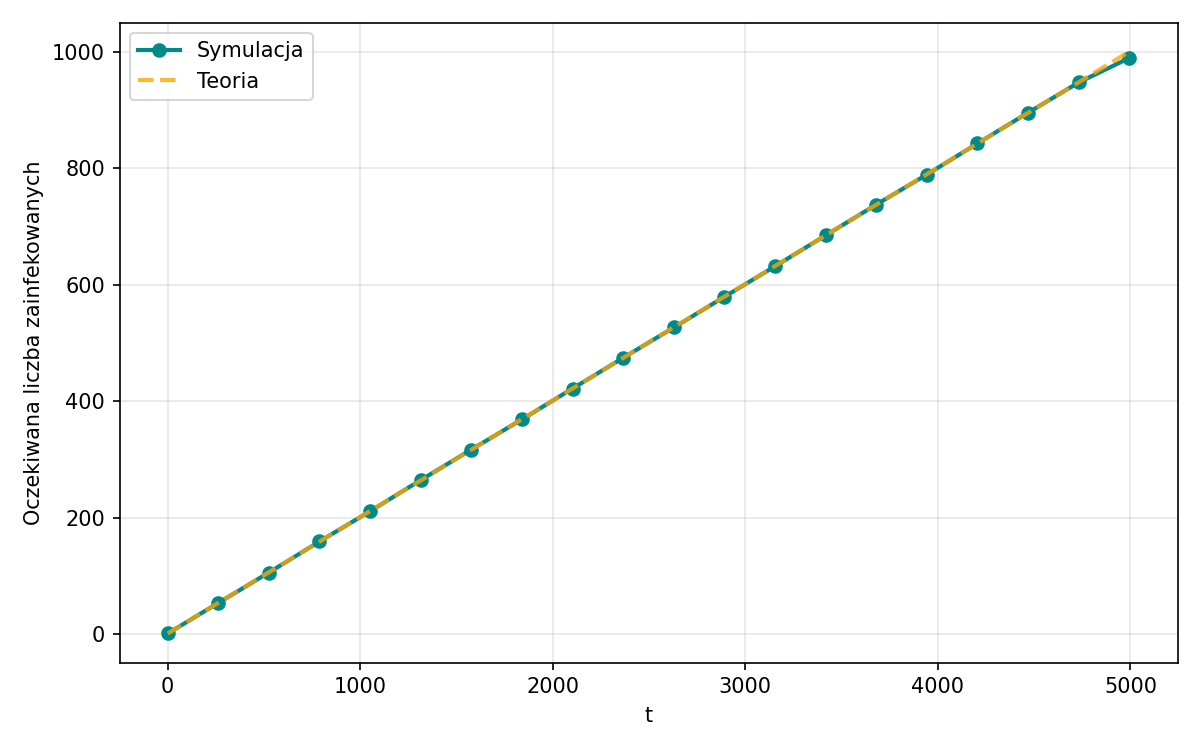
\includegraphics[width=1\textwidth]{../img/path/final_infection_expectations.png}
    \caption{$\mathbb{E}[Y_t]$ dla $\mathrm{P_n}$ w funkcji $t$}
\end{figure}
\begin{figure}[ht!]
    \centering
    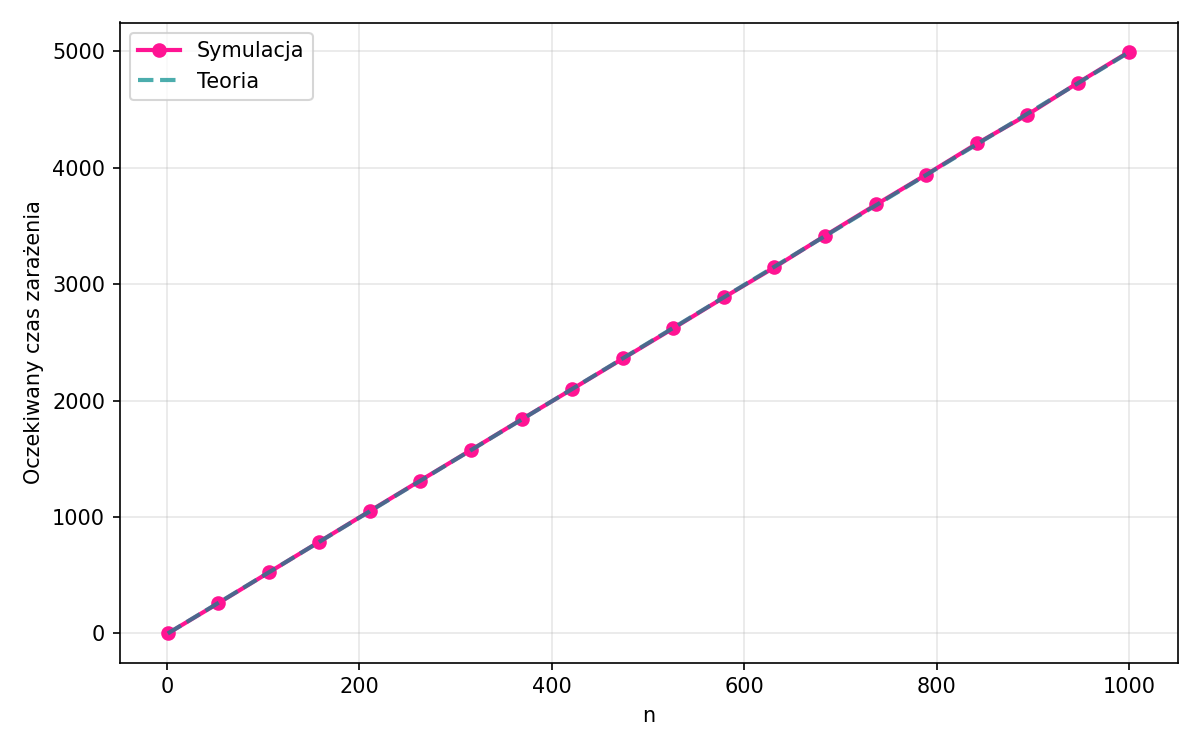
\includegraphics[width=1\textwidth]{../img/path/full_infection_expectation.png}
    \caption{$\mathbb{E}[Z]$ dla $\mathrm{P_n}$ w funkcji $n$}
\end{figure}
Wyniki eksperymentu niemal idealnie pokrywają się z przewidywanymi kształtami, to jest $1+tp$ dla $\mathbb{E}[Y_t]$ oraz $\frac{n-1}{p}$ dla $\mathbb{E}[Z]$.


\section{Grafy gwiezdne}

Następnie rozpatrzmy rodzinę grafów gwiazd $\mathrm{S}_n$. Niech źródłem będzie centralny wierzchołek grafu, to jest $s=0$. Propagacja rozchodzi się tutaj po każdym ramieniu gwiazdy niezależnie. Stąd mamy $X_v \sim \mathrm{Geo}(p)$ dla każdego $v\in\{1,2,\dots,n\}$. Ponadto zmienne $X_1,X_2,\dots,X_n$ są od siebie niezależne. Mamy więc
\[
    \mathbb{E}[X_v]=\frac{1}{p}, \quad \mathrm{Var}[X_v]=\frac{1-p}{p^2}
\]

Kwestia $Y_t$ jest również dość prosta. Skoro propagacja działa na każdym wierzchołku niezależnie to zmienna $Y_t$ jest wynikiem $n$ prób Bernoulliego. Sukces pojedynczej próby to prawdopodobieństwo, że zmienna $X_v$ o rozkładzie geometrycznym po conajwyżej $t$ jednostkach czasu osiągnie swój sukces. A więc jest to $\mathbb{P}[X_v\le t]=1-q^t$. W takim razie mamy
\[
    Y_t = 1 + B_t, \quad B_t \sim \mathrm{Bin}(n, 1-q^t)
\]
Stąd oczywiście otrzymujemy 
\[
    \mathbb{E}[Y_t] = 1 + n\cdot (1-q^t)
\]

Przejdźmy teraz do zmiennej $Z$. Mamy $Z=\max\{X_1,X_2,\dots,X_n\}$. Skoro zmienne te są IID, to z \Cref{fact:max_CDF} mamy 
\[
    \mathbb{P}[Z\le t] = {(1-q^t)}^n
\]
Policzmy teraz wartość oczekiwaną całkowitego zainfekowania grafu. 
\begin{equation*}
\begin{aligned}
\mathbb{E}[Z] 
&= \sum_{k=1}^{\infty} \mathbb{P}[Z\ge k] 
 = \sum_{k=1}^{\infty} 1 - \mathbb{P}[Z\le k-1]
 = \sum_{k=1}^{\infty}  1 - {(1-q^{k-1})}^n  \\
&= \sum_{k=0}^{\infty}  1 - {(1-q^k)}^n 
 = \sum_{k=0}^{\infty} \Big( 1 - \sum_{j=0}^{n} \binom{n}{j} {(-1)}^j q^{kj} \Big) \\
&= \sum_{k=0}^{\infty} \sum_{j=1}^{n} \binom{n}{j} {(-1)}^{j+1} q^{kj} = \sum_{j=1}^{n} \sum_{k=0}^{\infty} \binom{n}{j} {(-1)}^{j+1} {(q^j)}^k \\
&= \sum_{j=1}^{n} \binom{n}{j} \frac{{(-1)}^{j+1}}{1-q^j}
\end{aligned}
\end{equation*}
Nie jest to jednak przyzwoity wynik i nie ma postaci zwartej. Spróbujmy zatem wyznaczyć asymptotykę $\mathbb{E}[Z]$. Mamy $\mathbb{E}[Z] = \sum_{k=0}^{\infty}  1 - {(1-q^k)}^n$. `\ '\cref{inequality:approximation_of_sum_by_an_integral} umożliwia oszacowanie tej sumy. Połóżmy $f(x) = 1 - {(1 - e^{-\lambda x})}^n$ gdzie $\lambda = -\log(q)$. Oczywiście $f(0)=1$, $f(\infty)=0$ oraz $f$ jest malejąca a więc
\[
    \int_{0}^{\infty} f(x) \; \mathrm{d}x \le \mathbb{E}[Z] \le  1 + \int_{0}^{\infty} f(x) \; \mathrm{d}x
\]
Podstawiamy $u = 1 - e^{-\lambda x}$. Wtedy $\mathrm{d}u = \lambda e^{-\lambda x} \; \mathrm{d}x$,  a więc $\mathrm{d}x = \frac{1}{\lambda}\cdot\frac{1}{1-u} \; \mathrm{d}u$. Ponadto $u(0) = 0$, $u(\infty) = 1$ (bo $\lambda > 0$). Zatem całka ma postać:
\[
 \frac{1}{\lambda} \int_{0}^{1} \frac{1 - u^n}{1 - u} \; \mathrm{d}u
= \frac{1}{\lambda} \int_{0}^{1} \sum_{j=0}^{n-1} u^j \; \mathrm{d}u
= \frac{1}{\lambda} \sum_{j=0}^{n-1} \frac{1}{j+1}
= \frac{H_n}{\lambda}
\]
Zauważmy, że $-\log(q)=\log(\frac{1}{1-p})$ a więc ostatecznie dostajemy:
\[
    \frac{H_n}{\log(\frac{1}{1-p})} \le \mathbb{E}[Z] \le \frac{H_n}{\log(\frac{1}{1-p})} + 1
\]
Stąd mamy asymptotyczny przewidywany czas zarażenia grafu $\mathrm{S}_n$:
\[
    \mathbb{E}[Z] \sim \frac{H_n}{\log(\frac{1}{1-p})}
\]

Przeprowadźmy teraz symulacje. Ustalmy $p=0.2$, $n=1000$. Dla każdego $t\in\{1, 2, \dots, \log(n)\}$ wykonajmy $2000$ powtórzeń propagacji na $\mathrm{S}_n$. Potem dla $n\in\{1,2,\dots,1000\}$ tak samo dla $\mathbb{E}[Z]$. 
\begin{figure}[!ht]
    \centering
    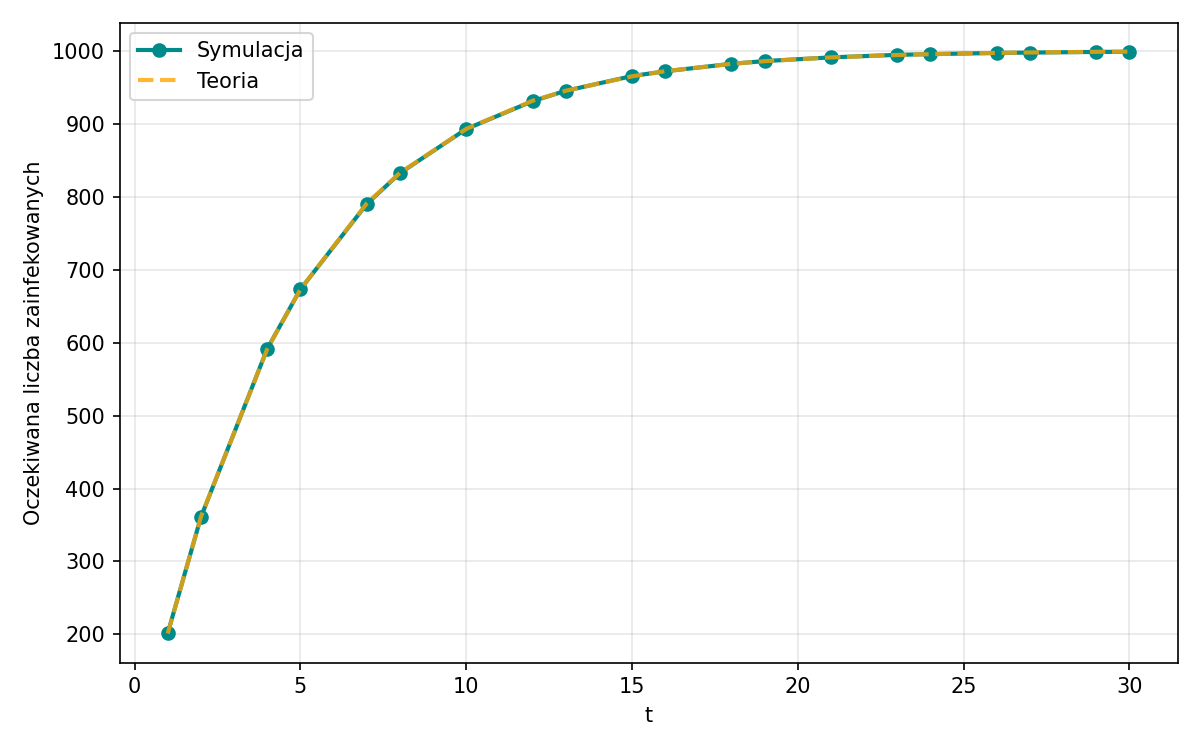
\includegraphics[width=1\textwidth]{../img/star/final_infection_expectations.png}
    \caption{$\mathbb{E}[Y_t]$ dla $\mathrm{S_n}$ w funkcji $t$}
\end{figure}
\begin{figure}[!ht]
    \centering
    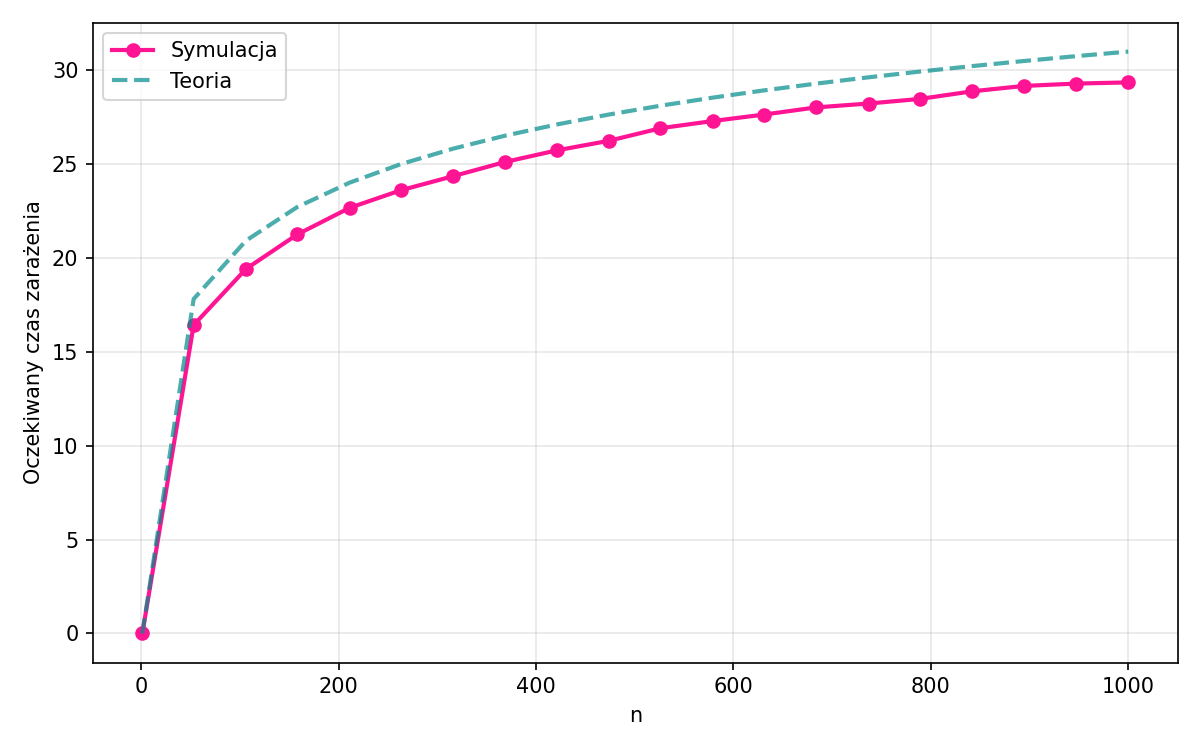
\includegraphics[width=1\textwidth]{../img/star/full_infection_expectation.png}
    \caption{$\mathbb{E}[Z]$ dla $\mathrm{S_n}$ w funkcji $n$}
\end{figure}
Dla $\mathbb{E}[Y_t]$ po raz kolejny mamy idealne dopasowanie. Dla $\mathbb{E}[Z]$ zaś numeryczna wartość jest o około $1$ mniejsza niż przewidywana, co jest dobrym wynikiem.


\section{Ograniczenia na czas zarażenia}

Po rozważeniu dwóch rodzin grafów dostrzegamy znaczną różnicę w wartościach oczekiwnaych zmiennych $Y_t$ oraz $Z$. Dla grafów ścieżkowych minimalna liczb rund potrzebnych do zainfekowania całego grafu wynosi $t=n-1$ natomiast dla gwiazd jest to zaledwie $t=1$. Widzimy, że w pewnym sensie najlepszy przypadek sprzyjający szybkiej propagacji jest taki, w którym źródło $s$ jest połączone z wszyskimi pozostałymi wierzchołkami grafu. Z drugiej strony najgorsza sytuacja ma miejsce, jeśli istnieje daleko oddalony węzeł, szczególnie z mało liczbą ścieżek do niego prowadzących, tak jak dla grafów ścieżkowych. Teraz postaramy się uogólnić tę obserwację. 

\begin{theorem}\label{theorem:montonicity_of_total_infection}
Niech $G=(V,E)$ będzie grafem spójnym a $G'=(V,E')$ spójnym podgrafem $G$. Załóżmy, że $\mathbf{X}$ jest procesem stochastycznym w modelu SI na $G$ oraz $G'$ jednocześnie z tym samym źródłem $s\in V$. Jeśli przez $X_v'$, $Y_t'$ oraz $Z'$ oznaczymy zmienne losowe w $G'$ odpowiadające tym w  $G$ to zachodzą następujące nierówności:
\[
    X_v \le X_v', \quad Y_t \ge Y_t', \quad Z\le Z'
\] 
\end{theorem}
\begin{proof}
Oznaczmy przez $\mathcal{I}_t$ zainfekowane wierzchołki w $G$ a przez $\mathcal{I}_t'$ w $G'$. Wtedy $\mathcal{I}'_t\subseteq\mathcal{I}_t$ dla dowolnego $t\in\mathbb{N}$. Ustalmy $v\in V$. Niech $X_v'=a$. Wtedy $v\in\mathcal{I}_a'$ jak i $v\in\mathcal{I}_a$. Stąd $X_v\le a=X_v'$. Ustalmy teraz $t\in\mathbb{N}$. Oczywiście skoro $\mathcal{I}_t'\subseteq\mathcal{I}_t$ to i $|\mathcal{I}_t'|\le|\mathcal{I}_t|$ a co za tym idzie $Y_t'\le Y_t$. Dalej niech $Z' = b$. Wtedy $\mathcal{I}'_b =V$ a więc $V\subseteq \mathcal{I}_t$. Zatem $\mathcal{I}_b = V$ i $Z\le b=Z'$. 
\end{proof}

Intuicyjnie sprawa jest oczywista. Mając mniej krawędzi w grafie potrzebujemy więcej czasu na rozprzestrzenienie się w nim informacji. W praktyce oznacza to, że jeżeli znamy średni czas zainfekowania dowolnego podgrafu $G$ to znamy ogarniczenie górne na czas dla całego grafu. Postarajmy się teraz oszacować sensownie z góry wartość $\mathbb{E}[Z]$ dla dowolnego grafu.

\begin{theorem}\label{theorem:upper_bound_on_EZ}
Niech $G=(V,E)$ będzie grafem o $n$ wierzchołkach zaś $s\in V$ będzie ustalonym źródłem. Oznaczmy $\lambda=\log(\frac{1}{1-p})$ oraz $h = \epsilon(s)$. Wtedy zachodzi
\[
    \mathbb{E}[Z] \le h  + \frac{h}{\lambda} \cdot \Big(\log\Big(\frac{n-1}{h}\Big) + 1\Big)
\]
\end{theorem}

\begin{proof}
Dla $0\le j \le h$ kładziemy $A_j = \{v \in V : \mathrm{d}(s,v) = j\}$ oraz $a_j= |A_j|$. Oczywiście $a_0=1$ a więc $a_1+\cdots+ a_h = n -1 $. Dalej zdefiniujmy zmienne losowe $T_j = \min\{t\in\mathbb{N} : A_j \subseteq \mathcal{I}_t\}$. Zmienna $T_j$ określa czas potrzebny do zainfekowania wierzchołków oddalonych o $j$ od źródła. Udowodnijmy teraz przydatny lemat.

\begin{lemma}\label{lemma:helper_lemma}
Niech $U_j = T_j - T_{j-1}$ dla $1 \le j \le h$. Wtedy:
\[
    \mathbb{E}[U_j] \le \frac{H_{a_j}}{\lambda} + 1
\]
\end{lemma}
\begin{proof}
$U_j$ to czas potrzebny na zarażenie wierzchołków $A_j$ podczas gdy $A_{j-1}$ są już zarażone. Wybierzmy podgraf $G'$ w taki sposób, żeby każdy wierzchołek z $A_j$ był połączony dokładnie jedną krawędzią z którymś z wierzchołków ze zbioru $A_{j-1}$. Wtedy rozkład propagacji na $G'$ jest izomorficzny z tym dla $\mathrm{S}_{a_j}$ bo $a_j=|A_j|$. Z \Cref{theorem:montonicity_of_total_infection} wnioskujemy, że zmienna $U_j$ jest ograniczona przez całkowity czas zarażenia grafu gwiazdy. Wartośc oczekiwana w tym drugim przypadku jest mniejsza niż $\frac{1}{\lambda}H_{a_j} + 1$. Z monotoniczności wartości oczekiwanej dostajemy porządany wynik.
\end{proof}

Wróćmy do udowadniania ograniczenia na $\mathbb{E}[Z]$. Mamy $T_h = \sum_{j=1}^{h} U_j$ a więc:
\begin{equation*}
\begin{aligned}
\mathbb{E}[Z] 
&= \mathbb{E}[T_h] 
  = \mathbb{E}\Big[\sum_{j=1}^{h} U_j\Big] 
  = \sum_{j=1}^{h} \mathbb{E}[U_j] 
  \le \sum_{j=1}^{h} \frac{H_{a_j}}{\lambda} + 1 \\
&= h + \frac{1}{\lambda} \sum_{j=1}^{h} H_{a_j} 
  \le h + \frac{1}{\lambda} \sum_{j=1}^{h} 1 + \log(a_j) \\
&= h + \frac{h}{\lambda} \cdot \Big(1 + \sum_{j=1}^{h} \log(a_j) \Big) = h + \frac{h}{\lambda} \cdot \Big(1 + \log \Big(\prod_{j=1}^{h} a_j\Big)\Big)\\
&\le h + \frac{h}{\lambda} \cdot \Big(1 + \log \Big(\frac{1}{h} \sum_{j=1}^{h} a_j\Big) \Big) = h + \frac{h}{\lambda} \cdot \Big(1 + \log \Big(\frac{n-1}{h}\Big) \Big) \\
\end{aligned}
\end{equation*}
gdzie w linijce pierwszej wykorzystujemy \cref{lemma:helper_lemma}, w drugiej \cref{inequality:harmonic_upper_bound} a w piątej nierówność między średnimi (\ref{inequality:AM_GM}).
\end{proof}

Porównajmy przed chwilą udowodnione twierdzenie z poprzednimi wynikami. Dla rodziny $\mathrm{P}_n$ mamy $h = n - 1$. Dodatkowo korzystając z \Cref{inequality:log_vs_x} mamy
\[
    \mathbb{E}[Z] \le (n-1) \cdot \Big(1 + \frac{1}{p} \Big)
\]
Faktyczna wartość oczekiwana jest równa $\frac{n-1}{p}$ więc oszacowanie jest dość ostre. Z kolei dla rodziny $\mathrm{S}_n$ mamy $h=1$ oraz $n+1$ wierzchołków a więc
\[
    \mathbb{E}[Z] \le 1 + \frac{\log(n) + 1}{\log(\frac{1}{1-p})}
\]
Ponownie oszacowanie jest dość dokładne. Wynik ten zdaje się być dobry dla grafów rzadkich.


\section{Grafy cykliczne}

Przejdźmy teraz do grafów cyklicznych. W rozważaniach dla trójkąta, to jest $\mathrm{C}_3$ mogliśmy zauważyć, że cykl w tym grafie sprawiał trudności. W ogólnym przypadku nie jest lepiej. Rozważmy graf $\mathrm{C}_n$.Niech źródłem będzie wierzchołek $n$. Ustalmy wierzchołek $v\in\{1,2,\dots,n-1\}$. Niech $a=\min\{v,n-v\}$ oraz $b=\max\{v,n-v\}$. Oczywiście $a\le b$. Od źródła do tego wierzchołka są dwie ścieżki: jedna o długości $a$, druga o długości $b$. Propagacja rozchodzi się po nich równolegle i niezależnie. Dla $j\in \{1,2,\dots,n-1\} $ połóżmy $N_j\sim \mathrm{NegBin}(j,p)$. Zmienne te są niezależne. Mamy wtedy 
\[
    X_v \sim \min\{N_a, N_b\}
\]
Niech $F_j(t)$ będzie dystrybuantą zmiennej $N_j$. Z \Cref{fact:min_CDF} mamy 
\[
    \mathbb{P}[X_v\le t] = 1 - (1-F_a(t))\cdot(1-F_b(t))
\]
Nie ma co liczyć na wyznaczenie eleganckiej postaci na PMF czy CDF dla $X_v$. Postaramy się więc przybliżyć wartość oczekiwaną dla dużych $n$. Z centralnego twierdzenia granicznego możemy przybliżyć $N_a \approx A,\; N_b \approx B$ dla $ A\sim \mathcal{N}(\mu_a,\sigma^2_a),\; B \sim \mathcal{N}(\mu_b,\sigma^2_b)$ gdzie 
\[
    \mu_a=\frac{a}{p},\quad \sigma^2_a=\frac{aq}{p^2}, \quad \mu_b=\frac{b}{p},\quad \sigma^2_b=\frac{bq}{p^2}
\]
Zatem mamy
\[
    \mathbb{E}[X_v] \approx \mathbb{E}[\min\{A,B\}]=\mathbb{E}\Big[\frac{A+B-|A-B|}{2}\Big]=\frac{\mathbb{E}[A]+\mathbb{E}[B]-\mathbb{E}[|A-B|]}{2}
\]
Połóżmy $C=A-B$. Korzystając z \Cref{fact:sum_of_normal_RV} mamy $C \sim \mathcal{N}(\mu_a-\mu_b,\sigma_a^2+\sigma_b^2)$. Oznaczmy $\eta=\mu_a-\mu_b$ oraz $\xi=\sqrt{\sigma_a^2+\sigma_b^2}$. Potrzebujemy teraz następującego lematu:
\begin{lemma}\label{lemma:abs_normal_E}
Niech $X \sim \mathcal{N}(\mu,\sigma^2)$. Wtedy
\[
    \mathbb{E}[|X|] = 2\sigma\cdot \varphi\Big(\frac{\mu}{\sigma}\Big)+\mu\cdot (2\mathbf{\Phi}\Big(\frac{\mu}{\sigma}\Big)-1)
\]    
\end{lemma}
\begin{proof}
\[
    \mathbb{E}[|X|]= \int_{-\infty}^{\infty} \frac{|x|}{\sigma}\varphi\Big(\frac{x-\mu}{\sigma}\Big) \; \mathrm{d}x = \int_{0}^{\infty} \frac{x}{\sigma}\varphi\Big(\frac{x-\mu}{\sigma}\Big) \; \mathrm{d}x - \int_{-\infty}^{0} \frac{x}{\sigma}\varphi\Big(\frac{x-\mu}{\sigma}\Big) \; \mathrm{d}x
\]
Oznaczmy $c=\frac{\mu}{\sigma}$ oraz podstawmy $z=\frac{x-\mu}{\sigma}$. Zatem $x=\mu+\sigma z$, $\mathrm{d}{x}=\sigma \mathrm{d}{z}$. Dla $x>0$ mamy $z>-c$ zaś dla $x<0$ mamy $z<-c$. Otrzymujemy więc
\begin{align*}
&\int_{-c}^{\infty} (\mu+\sigma z)\varphi(z)\,\mathrm{d}z 
 - \int_{-\infty}^{-c} (\mu+\sigma z)\varphi(z)\,\mathrm{d}z \\[0.3em]
&= \mu \!\int_{-c}^{\infty} \!\varphi(z)\,\mathrm{d}z
   + \sigma \!\int_{-c}^{\infty} \!z\varphi(z)\,\mathrm{d}z
   - \mu \!\int_{-\infty}^{-c} \!\varphi(z)\,\mathrm{d}z
   - \sigma \!\int_{-\infty}^{-c} \!z\varphi(z)\,\mathrm{d}z \\[0.3em]
&= \mu\!\Big(\!\int_{-c}^{\infty}\!\varphi(z)\,\mathrm{d}z 
   - \!\int_{-\infty}^{-c}\!\varphi(z)\,\mathrm{d}z\!\Big)
   + \sigma\!\Big(\!\int_{-c}^{\infty}\!z\varphi(z)\,\mathrm{d}z 
   - \!\int_{-\infty}^{-c}\!z\varphi(z)\,\mathrm{d}z\!\Big) \\[0.3em]
&= \mu\!\Big(\!\int_{-\infty}^{\infty}\!\varphi(z)\,\mathrm{d}z 
   - 2\!\int_{-\infty}^{-c}\!\varphi(z)\,\mathrm{d}z\!\Big)
   + \sigma\!\Big(-\varphi(z)\big|_{-c}^{\infty}
   + \varphi(z)\big|_{-\infty}^{-c}\Big) \\[0.3em]
&= \mu\cdot\!\Big(1 - 2\mathbf{\Phi}(-c)\Big)
   + \sigma\cdot\!\Big(-\varphi(\infty)+\varphi(-c)+\varphi(-c)-\varphi(-\infty)\Big) \\[0.3em]
&= \mu\cdot\!\Big(2\mathbf{\Phi}(c)-1\Big) + 2\sigma\cdot\,\varphi(c)
\end{align*}
gdzie skorzystaliśmy z tożsamości $\mathbf{\Phi}(-x)=1-\mathbf{\Phi}(x)$, $\varphi(-x)=\varphi(x)$, \\ $\varphi(\pm\infty)=0$, $\int_{-\infty}^{\infty}\varphi(x) \;\mathrm{d}x = 1$ oraz $\int x\varphi(x)\;\mathrm{d}x=-\varphi(x)$.
\end{proof}

Z \Cref{lemma:abs_normal_E} dostajemy $\mathbb{E}[C]=2\xi\cdot \varphi\Big(\frac{\eta}{\xi}\Big)+\eta\cdot (2\mathbf{\Phi}\Big(\frac{\eta}{\xi}\Big)-1)$. Ostatecznie 
\begin{align*}
\mathbb{E}[X_v] \approx {} &
 \tfrac{1}{2}\!\Big(\mu_a+\mu_b
 -2\xi\,\varphi\!\Big(\tfrac{\eta}{\xi}\Big)
 -\eta\!\Big(2\mathbf{\Phi}\!\Big(\tfrac{\eta}{\xi}\Big)-1\Big)\!\Big) \\[0.4em]
={} &
 \tfrac{\mu_a+\mu_b}{2}
 -\xi\,\varphi\!\Big(\tfrac{\eta}{\xi}\Big)
 -(\mu_a-\mu_b)\!\Big(\mathbf{\Phi}\!\Big(\tfrac{\eta}{\xi}\Big)-\tfrac{1}{2}\Big) \\[0.4em]
={} &
 \mu_a\!\Big(1-\mathbf{\Phi}\!\Big(\tfrac{\eta}{\xi}\Big)\Big)
 +\mu_b\,\mathbf{\Phi}\!\Big(\tfrac{\eta}{\xi}\Big)
 -\eta\,\varphi\!\Big(\tfrac{\eta}{\xi}\Big)
\end{align*}

Przenalizujmy teraz zachowanie asymptotyczne otrzymanego wyrażenia. Skoro $a+b=n$ to niech $a=rn$, $b=(1-r)n$ dla pewnego $r\in(0;1)$. Dalej 
\[
    \frac{\eta}{\xi}=\frac{\mu_a-\mu_b}{\sqrt{\sigma_a^2+\sigma_b^2}}=\frac{\frac{a}{p}-\frac{b}{p}}{\sqrt{\frac{aq}{p^2}+\frac{bq}{p^2}}}=\frac{(2r-1)\sqrt{n}}{\sqrt{q}}
\]
Musimy rozważyć dwa przypadki.

Jeśli $a<b$, co za tym idzie $r<\frac{1}{2}$ to $\frac{\eta}{\xi}\to -\infty$ wraz z $n\to \infty$. Wtedy też $\varphi\Big(\frac{\eta}{\xi}\Big)\to 0$ oraz $\mathbf{\Phi}\Big(\frac{\eta}{\xi}\Big)\to 0$ a więc $\mathbb{E}[X_v] \to \frac{a}{p}$. 

Zaś gdy $a=b$ to $r=\frac{1}{2}$ jak i  $\frac{\eta}{\xi}=0$. Wiemy, że $\varphi(0)=\frac{1}{\sqrt{2\pi}}$ oraz $\mathbf{\Phi}(0)=\frac{1}{2}$. Wstawiając otrzymamy $\mathbb{E}[X_v] \to \frac{n}{2p}-\frac{\sqrt{np}}{p\sqrt{2\pi}}$. 
Podsumowując mamy następujący wynik:
\[
    \mathbb{E}[X_v] \sim \frac{\min\{v,n-v\}}{p}
\]
Jest to całkowicie zgodne z intuicją. Wierzchołki w grafie $\mathrm{C}_n$ zachowują się podobnie jak w grafach $\mathrm{P}_n$.

W celu wyznaczenie rozkładu $Y_t$ dokonajmy obserwacji, że gdy dwie drogi zarażania spotkają się to propagacja dobiega końca. Każda z tych dróg jak w przypadku grafu ścieżkowego ma rozkład dwumianowy. Możemy zapisać zatem
\[
    Y_t \sim \min\{n, 1+ L_t + R_t\}, \quad L_t,R_t\sim \mathrm{Bin}(t,p)
\] 
Z \Cref{fact:sum_of_bin_RV} mamy $L_t+R_t\sim\mathrm{Bin}(2t,p)$. Widzimy zatem, że rozkład $Y_t$ dla grafu $\mathrm{C}_n$ pokrywa się ze zmienną $Y_{2t}$ dla grafów typu $\mathrm{P}_n$. Z wcześniejszego wyniku dla grafów ścieżek dostajemy
\[
    \lim_{n\to\infty} \mathbb{E}[Y_t] = 1+2tp
\]

Teraz możemy wyznaczyć $\mathbb{E}[Z]$. Dla $n$ patrzystego najdalej oddalony wierzchołek od źródła to $\frac{n}{2}$ a dla $n$ nieparzystego to $\lfloor \frac{n\pm 1}{2}\rfloor$. Asymptotycznie nie ma to znaczenia, możemy przyjąć $v=\frac{n}{2}$. Stąd
\[
    \mathbb{E}[Z] \approx \mathbb{E}[X_{\frac{n}{2}}] \approx \frac{n}{2p}-\frac{\sqrt{np}}{p\sqrt{2\pi}}
\]

Również intuicyjny wynik. Aby się upewnić czy nie przesadziliśmy z szacowanie zwrócmy się ku symulacji. Dla $p=0.2$, $n\in\{3,4,\dots, 1000\}$ policzmy wartość oczekiwaną całkowitego zarażenia po razy $2000$ razy. Z wykresu widzimy, że empiryczny wynik pokrywa się asymptotycznie z teoretycznym.
\begin{figure}[!ht]
    \centering
    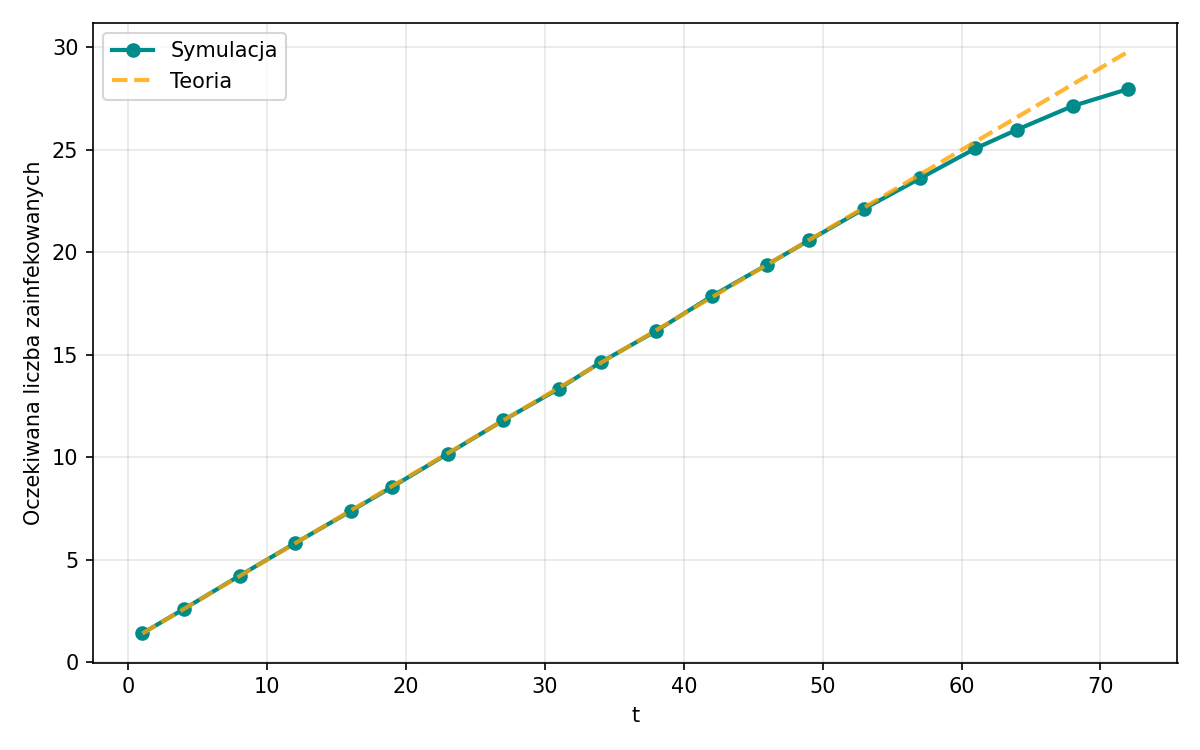
\includegraphics[width=1\textwidth]{../img/cycle/final_infection_expectations.png}
    \caption{$\mathbb{E}[Y_t]$ dla $\mathrm{C_n}$ w funkcji $t$}
\end{figure}
\begin{figure}[!ht]
    \centering
    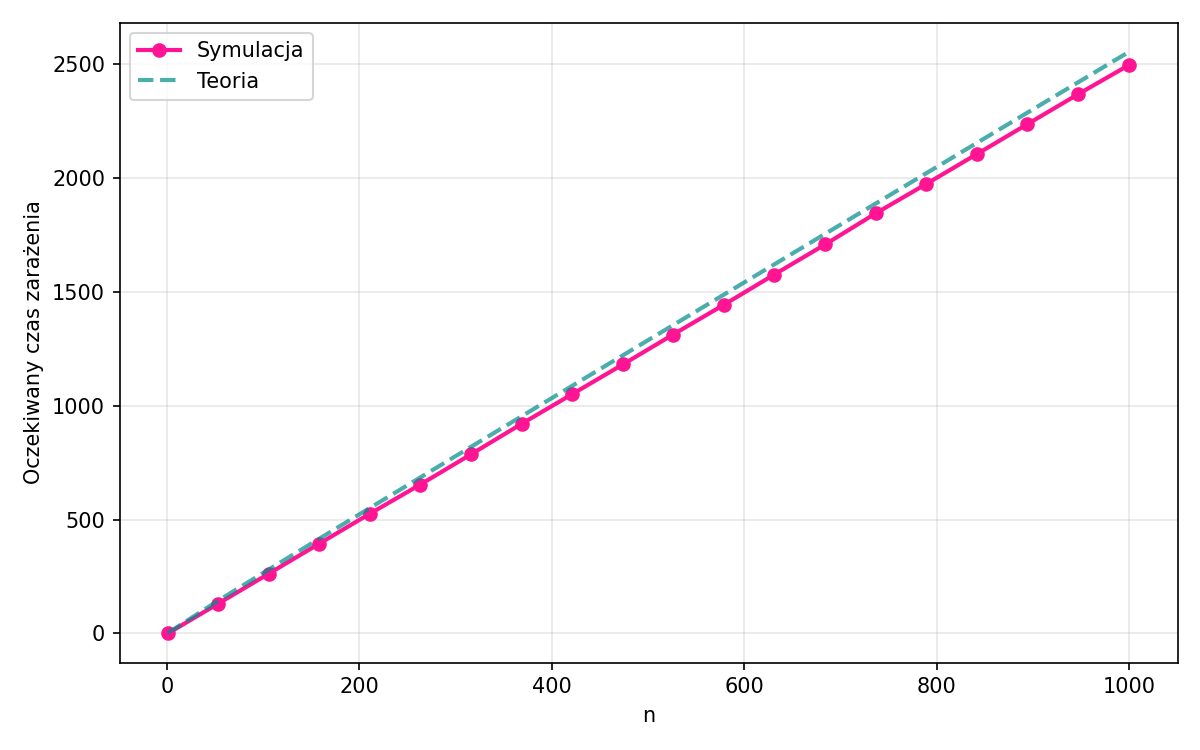
\includegraphics[width=1\textwidth]{../img/cycle/full_infection_expectation.png}
    \caption{$\mathbb{E}[Z]$ dla $\mathrm{C_n}$ w funkcji $n$}
\end{figure}


\section{Grafy pełne}

Graf pełny $\mathrm{K}_n$ intuicyjnie powinien mieć najszybszą propagację ze względu na maksymalną liczbę krawędzi. Za źródło możemy przyjąć dowolny wierzchołek $s\in V$ ze względu na symetrie. Początkowo rozkład $X_v$ pokrywa się z rozkładem gwiazdy natomiast w każdej kolejnej rundzie mocno się komplikuje. Zachodzi bowiem $Y_t=a$ to $\mathbb{P}[X_v = t+1 | Y_t = a] = 1 - q^a$. Nie mamy co liczyć na jakiekolwiek sensowne wyznaczenie rozkładu $X_v$. Podejdźmy do problemu narazie heurystycznie. Zauważmy, że jeśli $Y_1=a$ to rozkład zmiennej $Y_2$ wynosi $Y_2 = a + B$ dla $B \sim \mathrm{Bin}(n-a, 1-q^n)$. Zatem 
\[
    \mathbb{E}[Y_2\mid Y_1 = a] = n\cdot (1-q^a) + aq^a
\]
Mamy $Y_1\sim \mathrm{Bin}(n-1,p)$ oraz $\mathbb{E}[Y_1]=1+(n-1)p$. Możemy również założyć, że również $a \approx \mathbb{E}[Y_1]$ a co za tym idzie 
\[
    \mathbb{E}[Y_2\mid Y_1 = a] \approx n(1-q^{1+(n-1)p})+(1+(n-1)p)q^{1+(n-1)p} 
\]
Jeśli $n\to\infty$ to wyrażenie to jest bliskie $n$. Spodziewamy się zatem, że zaledwie po dwóch rundach cały graf $\mathrm{K}_n$ będzie zainfekowany. Zweryfikujmy teraz ten heurystyczny argument symulacją w Pythonie. Ustalmy $p=0.2$ i dla $n\in\{2,3,\dots,1000\}$ odpalmy propagację. 
\begin{figure}[!ht]
    \centering
    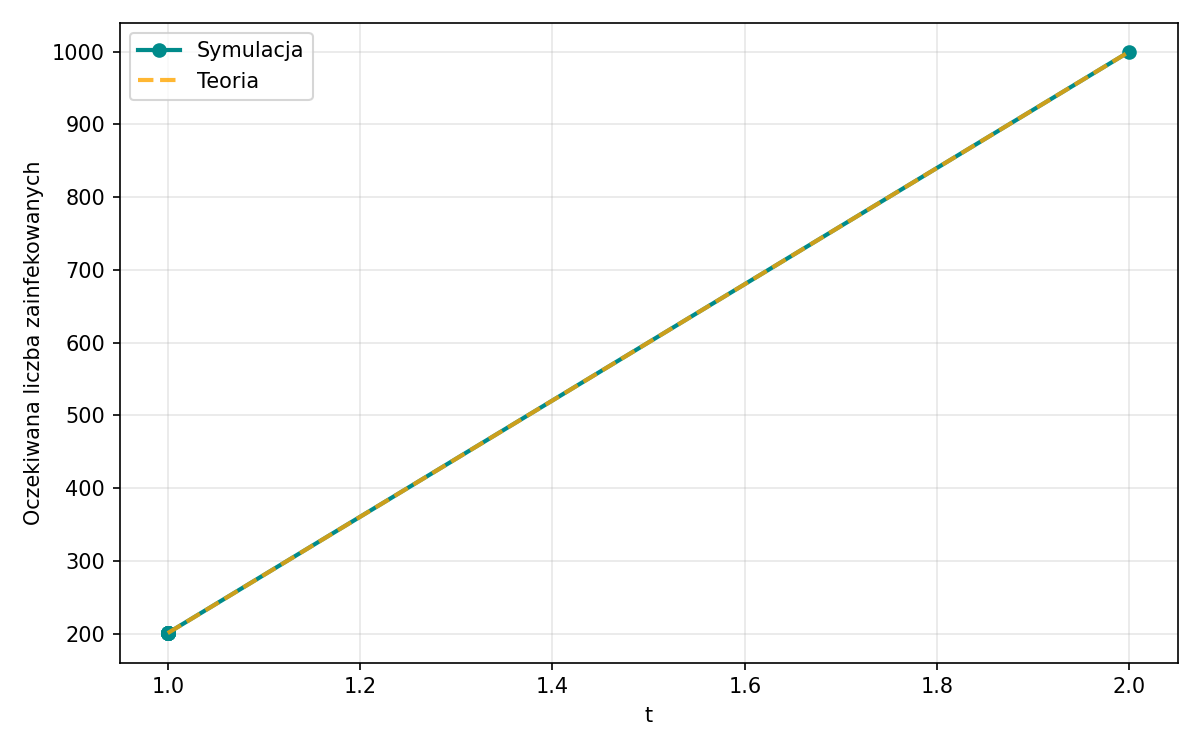
\includegraphics[width=1\textwidth]{../img/complete/final_infection_expectations.png}
    \caption{$\mathbb{E}[Y_t]$ dla $\mathrm{K_n}$ w funkcji $t$}
\end{figure}
\begin{figure}[!ht]
    \centering
    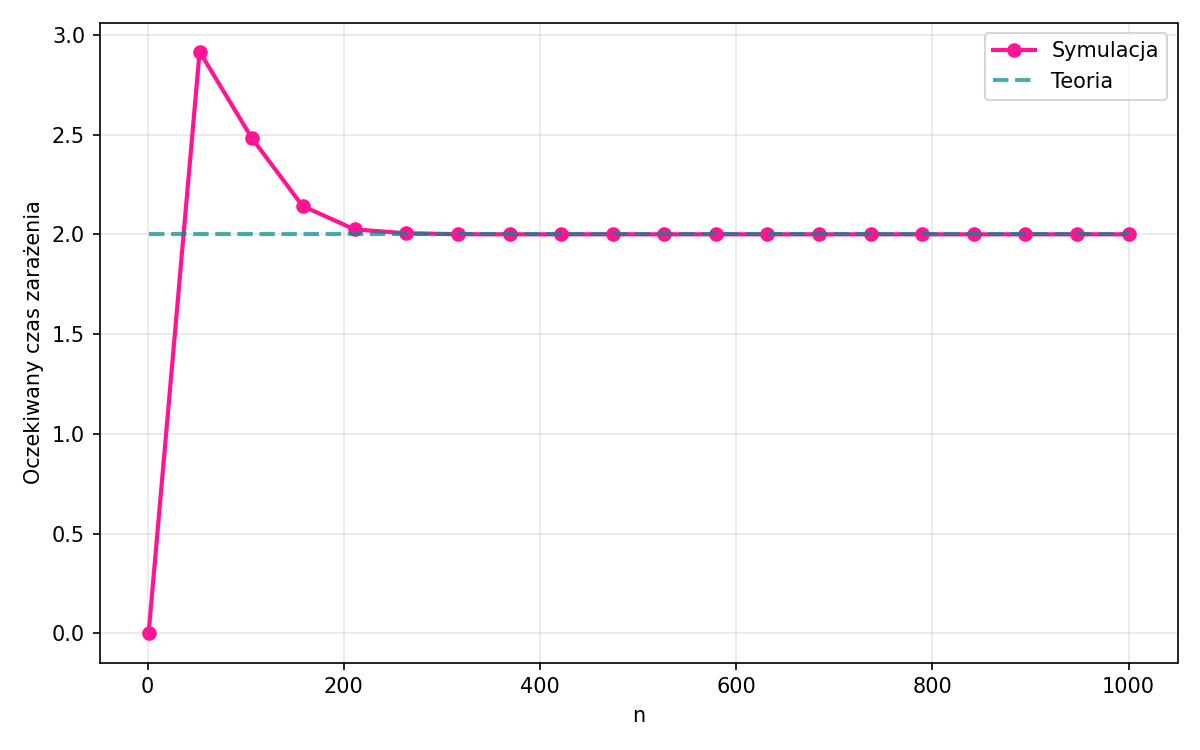
\includegraphics[width=1\textwidth]{../img/complete/full_infection_expectation.png}
    \caption{$\mathbb{E}[Z]$ dla $\mathrm{K_n}$ w funkcji $n$}
\end{figure}
Widzimy, że dla $n>200$ mamy $\mathbb{E}[Z] \approx 2$. Możemy więc wysunąć hipotezę: Dla grafu $\mathrm{K}_n$ mamy:
\[
    \lim_{n\to\infty} \mathbb{E}[Z] = 2
\]
Postarajmy się ją teraz udowodnić. Żeby to zrobić najpierw wyznaczmy asymptotyke $\mathbb{E}[Y_2]$. Oznaczamy $U=Y_1=1+W$ gdzie $W\sim\mathrm{Bin}(n-1,p)$. Z prawa całkowitej wartości oczekiwanej mamy
\[
    \mathbb{E}[Y_2] = n\cdot (1-\mathbb{E}[q^U])+\mathbb{E}[Uq^U]
\]
Musimy wyznaczyć $\mathbb{E}[q^U]$ jak i $\mathbb{E}[Uq^U]$. 
\begin{lemma}\label{lemma:binomial_PGF}
Niech $X \sim \mathrm{Bin}(m, p)$. Wtedy
\[
    \mathbb{E}[z^X]={(q+pz)}^m, \quad \mathbb{E}[Xz^X]=mpz{(q+pz)}^{m-1}
\]    
\end{lemma}
\begin{proof}
Do obliczenia tych wartości posłuży nam \cref{summ:binomial_0} jak i \cref{summ:binomial_1}.
\[
    \mathbb{E}[z^X] = \sum_{k=0}^{m} z^k \cdot \binom{m}{k}p^k q^{m-k} = \sum_{k=0}^{m} \binom{m}{k}{(pz)}^k q^{m-k} = {(q+pz)}^m
\]    
\[
    \mathbb{E}[Xz^X] = \sum_{k=0}^{m} kz^k \binom{m}{k}p^k q^{m-k} = \sum_{k=0}^{m} k \binom{m}{k}{(pz)}^k q^{m-k} = mpz{(q+pz)}^{m-1} 
\]
\end{proof}

W naszym przypadku dostajemy 
\[
    \mathbb{E}[q^U]=\mathbb{E}[q^{1+W}]=q\cdot \mathbb{E}[q^W]=q{(q+pq)}^{n-1}=q^n{(1+p)}^{n-1}
\]
Dla drugiej wartości mamy zaś
\begin{equation*}
\begin{aligned}
\mathbb{E}[Uq^U] 
&= \mathbb{E}[(1+W)q^{1+W}] = q(\mathbb{E}[q^W]+\mathbb{E}[Wq^W]) \\
& = q(q^{n-1}{(1+p)}^{n-1}+(n-1)pq^{n-1}{(1+p)}^{n-2}) \\
&= q^n{(1+p)}^{n-2}(1+p+(n-1)p)=q^n{(1+p)}^{n-2}(1+np)
\end{aligned}
\end{equation*}
Podstawiając przed chwilą wyrażenia wzory do wzoru na $\mathbb{E}[Y_2]$ dostaniemy
\begin{equation*}
\begin{aligned}
\mathbb{E}[Y_2] 
&= n-nq^n{(1+p)}^{n-1}+q^n{(1+p)}^{n-2}(1+np)= \\
&= n-(n-1)q^n{(1+p)}^{n-2}=n-(n-1){(1+p)}^{-2}{(1-p^2)}^n
\end{aligned}
\end{equation*}
Połóżmy $\varepsilon_n=(n-1){(1+p)}^{-2}{(1-p^2)}^n$. Wtedy $\mathbb{E}[Y_2]=n-\varepsilon_n$. Z nierówności Markova (\ref{inequality:Markov}) otrzymujemy $\mathbb{P}[Z\ge 3]=\mathbb{P}[n-Y_2\ge 1]\le \mathbb{E}[n-Y_2]=\varepsilon_n$. Dalej zauważmy, że $\mathbb{P}[Z=1]=p^{n-1}$ bo wszystkie próby zarażenia w rundzie pierwszej musiałby by się powieść. Ograniczmy teraz z dwóch stron $\mathbb{E}[Z]$. Z dołu mamy
\[
    \mathbb{E}[Z]=\sum_{k=1}^{\infty}\mathbb{P}[Z\ge k] \ge \mathbb{P}[Z\ge 1] + \mathbb{P}[Z\ge 2] = 1 + 1 - p^{n-1} = 2 - p^{n-1}
\]
Zajmijmy się teraz oszacowaniem górnym. Zauważmy, że graf $\mathrm{K}_n$ zawiera $\mathrm{P}_n$ jako podgraf. Ustalmy jeden z tych podgrafów. Niech $Z'$ będzie zmienną losową czasu całkowitego zarażenia dla tego podgrafu. Z \Cref{theorem:montonicity_of_total_infection} mamy $Z\le Z'$ a co za tym idzie $\mathbb{E}[Z^2] \le \mathbb{E}[{(Z')}^2]$. Przypomnijmy, że $Z' \sim \mathrm{NegBin}(n-1,p)$ a więc $\mathbb{E}[{(Z')}^2]=\frac{{(n-1)}^2+(n-1)q}{p^2}$. 
\begin{equation*}
\begin{aligned}
\mathbb{E}[Z] 
&= \sum_{k=1}^{\infty}\mathbb{P}[Z\ge k] = \mathbb{P}[Z\ge 1] + \mathbb{P}[Z\ge 2] + \sum_{k = 3}^{\infty} \mathbb{P}[Z\ge k]  \\
&= 1 + 1-p^{n-1} + \mathbb{E}[Z \cdot \mathbf{1}_{Z\ge 3}] \le 2 - p^{n-1} + \sqrt{\mathbb{E}[Z^2]}\sqrt{\mathbb{E}[\mathbf{1}_{Z\ge 3}]} \\
&\le 2 - p^{n-1} + \sqrt{\mathbb{E}[{(Z')}^2]}\sqrt{\mathbb{P}[Z\ge 3]} \\
&\le 2 - p^{n-1} + \sqrt{\frac{{(n-1)}^2+(n-1)q}{p^2}}\sqrt{\varepsilon_n}
\end{aligned}
\end{equation*}
gdzie wykorzystaliśmy nierówność Cauchy’ego-Schwarza (\ref{inequality:Cauchy_Schwarz}). Ostatecznie dostajemy 
\[
    2-p^{n-1}\le \mathbb{E}[Z] \le 2 - p^{n-1} + \sqrt{\frac{{(n-1)}^2+(n-1)q}{p^2}}\sqrt{\varepsilon_n}
\]
a zatem
\[
    \lim_{n \to \infty} \mathbb{E}[Z] = 2
\]
Jeżeli zaledwie po dwóch rundach cały graf jest poinformowany to rozkłady $X_v$ czy $Y_t$ nie są dla nas istotne. Spójrzmy jeszcze na oszacowanie, które otrzymamy stosując \cref{theorem:upper_bound_on_EZ} dla grafu pełnego. Wynosi ono $1 + \frac{\log(n-1) + 1}{\log(\frac{1}{1-p})}$. Ograniczenie to zdaje się nie być za dobre czego przyczną jest fakt, że $\mathrm{K}_n$ jest grafem gęstym.

\section{Drzewa}

Rozważmy drzewo $G = (V, E)$ oraz ustalony wierzchołek początkowy $s \in V$, 
który traktujemy jako korzeń drzewa. Dla $v\in V$ oznaczmy  $d_v=\mathrm{d}(s,v)$. Ustalmy $v\in V$. Skoro $G$ jest drzewem to istnieje dokładnie jedna ścieżka od $s$ do $v$, powiedzmy $s,v_1,\dots,v_k, v$. Ponieważ infekcja rozprzestrzenia się od korzenia $s$ wzdłuż krawędzi drzewa, 
każde zakażenie wymaga sukcesu w niezależnym doświadczeniu Bernoulliego o prawdopodobieństwie $p$.
W konsekwencji, aby infekcja dotarła z $s$ do $v$, 
musi wystąpić $\mathrm{d}_v$ kolejnych sukcesów. Zatem rozkład $X_v$ pokrywa się z rozkładem tej zmiennej dla grafu $\mathrm{P}_{d_v+1}$ na wierzchołkach $\{s,v_1,\dots,v_k, v\}$. Stąd 
\[
    X_v\sim \mathrm{NegBin}(\mathrm{d}_v,p)
\]
oraz
\[
    \mathbb{E}[X_v] = \frac{\mathrm{d}_v}{p}, \quad \mathrm{Var}[X_v] = \frac{\mathrm{d}_v\cdot(1 - p)}{p^2}
\]
\begin{lemma}\label{lemma:Formula_EYt}
Dla dowolnego $t\in\mathbb{N}$ wartość oczekiwana zmiennej $Y_t$ wyraża się wzorem
\[
    \mathbb{E}[Y_t] = \sum_{v\in V} \mathbb{P}[X_v \le t]
\]    
\end{lemma}

\begin{proof}
Mamy $Y_t=|\{v\in V: X_v \le t\}|$ zatem $Y_t=\sum_{v\in V}  \mathbf{1}_{\{X_v\le t\}}$. Nakładając na tą równość operator $\mathbb{E}$ otrzymujemy:
\[
    \mathbb{E}[Y_t] = \mathbb{E}\Big[ \sum_{v\in V}  \mathbf{1}_{\{X_v\le t\}}\Big]= \sum_{v\in V} \mathbb{E}[\mathbf{1}_{\{X_v\le t\}}] = \sum_{v\in V} \mathbb{P}[X_v \le t]
\]    
\end{proof}

Przejdźmy teraz to obliczania średniej liczby zainfekowanych wierzchołków w czasie $t$. Oznaczmy przez $F(t;m,p)$ dystrybuante zmiennej o rozkładzie $\mathrm{NegBin}(m,p)$. Z \Cref{lemma:Formula_EYt} otrzymujemy
\[
    \mathbb{E}[Y_t] = \sum_{v\in V} F(t; d_v, p)
\]
Połóżmy $a_j = |\{v\in V: d_v=j\}|$ dla $0\le j \le h$. Wtedy 
\[
    \mathbb{E}[Y_t] = \sum_{j=0}^{h} a_j\cdot F(t; j, p)
\]
Ponadto gdy $t<j\le h$ to $F(t; j, p)$, bo żaden wierzchołek w odległości od korzenia większej niż liczba rund nie może zostać zarażony. Możemy więc zmniejszyć granice sumowania 
\[
    \mathbb{E}[Y_t] = \sum_{j=0}^{\min\{h,t\}} a_j\cdot F(t; j, p)
\]

Oszacujmy teraz średni czas całkowity czas propagacji drzewa.
Niech $L=\{u_1,\dots, u_m\}$ będzie zbiorem liści w $G$. Wtedy mamy $Z = \max_{u\in L} X_{u}$.
Zauważmy, że $\epsilon(s) = \max_{u\in L} \mathrm{d}_{u}$ i jest to wysokość drzewa. Oznaczmy ją przez $h$. Z nierówności Jensena (\ref{inequality:Jensen}) otrzymujemy
\[
    \mathbb{E}[Z]=\mathbb{E}[\max_{u\in L} X_{u}] \ge \max_{u\in L} \mathbb{E}[X_{u}] = \max_{u\in L} \frac{\mathrm{d}_{u}}{p} = \frac{h}{p}
\]
Aby ogarniczyć $\mathbb{E}[Z]$ z góry skorzystamy z \Cref{theorem:upper_bound_on_EZ}:
\[
    \mathbb{E}[Z] \le h  + h \cdot \frac{\log(\frac{n-1}{h}) + 1}{\log(\frac{1}{1-p})}
\]

Ograniczenia te są różnych rzędów wielkości. Jednakże nie da się ich poprawić dla ogólnego drzewa znając tylko liczbę jego wierzchołków i wysokość. Ustalmy $n\in\mathbb{N}_+$ oraz $h\in\{1,2,\dots,n-1\}$ i poszukajmy drzew o $n$ wierzchołkach i wysokości $h$ osiągających zarówno dolne jak i górne ograniczenie na $\mathbb{E}[Z]$. Dla dolnej nierówności możemy wziąść drzewo składające się ze ścieżki długości $h$ oraz $n-1-h$ liści bezpośrednio przy korzeniu. Wtedy $\mathbb{E}[Z] \approx \frac{h}{p}$. Aby znaleść drzewo osiągające górne ograniczenie musimy wrócic do dowodu \Cref{theorem:upper_bound_on_EZ}. Udowadniając granicę na wartość oczekiwaną korzystamy z trzech nierówności. Pierwsza z nich to \cref{inequality:harmonic_upper_bound}. Jest ona bardzo ciasna a ponadto niezależy od grafu. Druga z nich to nierównośc między średnią arytmetyczną a geometryczną (\ref{inequality:AM_GM}). Aby uzyskać równość potrzebujemy mieć $a_1=\cdots=a_h$. Czyli innymi słowy, nasze drzewo ma tyle samo węzłów na każdej głebokości. Połóżmy $a_1=b$. Wtedy $hb=n-1$ a więc $b=\lfloor\frac{n-1}{h}\rfloor$. Na koniec zostaje nierówność wynikająca z \Cref{lemma:helper_lemma}. Sam lemat daje nierówność, której nie da się poprawić, co wiemy poprzez analize dla grafów gwiazd. Lecz dla drzewa będzie ona najmniej luźna, jeżeli każdy wierzchołek w warstwie $A_j$ będzie miał dokładnie jedną krawędź łaczącą go z wierzchołkiem w warstiwe $A_{j+1}$, gdzie $0\le j\le h-1$. Zatem drzewo składa się z korzenia oraz $b$ rozłącznych ścieżek, każda o długości $h$. I taki graf osiąga ograniczenie górne na $\mathbb{E}[Z]$. Widzimy zatem, że nasze ograniczenia nie są do poprawnienia bez dodatkowych parametrów grafu. Podsumowując możemy następująco szacować przewidywany czas całkowitego poinformowania drzewa o wysokości $h$:
\[
    \frac{h}{p} \le \mathbb{E}[Z] \le h  + h \cdot \frac{\log(\frac{n-1}{h}) + 1}{\log(\frac{1}{1-p})}
\]